\chapter{Methodology}

\section{Introduction to Sliding Mode Control}

Sliding Mode Control (SMC) is a well-established strategy within the broader category of sensor-based control techniques. It is recognized for its robustness in maintaining system stability, even when confronted with uncertainties and external disturbances\cite{Hoy2015}.Fundamentally, SMC belongs to a specific class of nonlinear control methods, with its distinctiveness arising from the discontinuity inherent in its control signals. By continually adjusting the sliding surface based on the system's real-time state, SMC compels the system to adhere to a predefined ``sliding mode'' trajectory. This capability ensures precise control over the system's behavior throughout the process. Additionally, SMC dynamically adapts the control input through feedback mechanisms, enabling the system to remain stable and consistently follow the desired trajectory, even under significant external perturbations \cite{Liu2012}.The sliding surface is a crucial concept in the entire strategy.


\section{Definition of the Sliding Surface}
Consider a general scenario where, in the system 
\[
\dot{x} = f(x), \quad x \in \mathbb{R}^n,
\]
there is a switching surface 
\[
s(x) = s(x_1, x_2, \dots, x_n) = 0.
\]

This switching surface divides the state space into two distinct regions: \(s > 0\) and \(s < 0\). The system's behavior in the vicinity of this surface can be categorized into three distinct cases, as illustrated in Figure \ref{FIG:1}.



\begin{figure}[H]
    \centering
    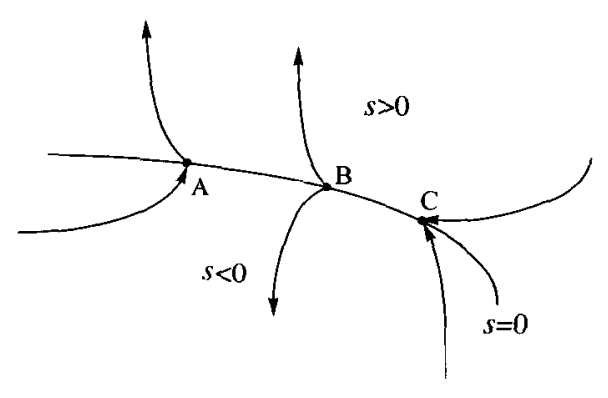
\includegraphics[scale=0.5]{1.png}
    \caption{Sliding Surface} % 图名称
    \label{FIG:1}
\end{figure}

The system trajectory demonstrates three unique types of behavior in proximity to the switching surface, where \(s = 0\).


1. \textbf{Regular Point}: The trajectory of the system moves toward the switching surface \( s = 0 \) and crosses through it, as represented by Point A.

2. \textbf{Starting Point}: The trajectory of the system approaches the switching surface \( s = 0 \) from both sides, converging to the surface without actually crossing it. This behavior is depicted by Point B.

3. \textbf{Endpoint}: The trajectory of the system reaches the switching surface \( s = 0 \) and remains on it, approaching from both sides without departing from the surface. This is illustrated by Point C.

    In sliding mode control, the starting point typically holds little significance, while the terminal point is of special importance. This is because once the system state point enters a particular region on the switching surface, all points within this region are considered terminal points. As the state point approaches this region, it is "attracted" to and remains within it. This region, located at \( s=0 \), is referred to as the "sliding mode region" or simply the "sliding region." The motion of the system within this region is known as "sliding motion."

 According to the sliding mode control requirements, all points in the sliding region should be treated as terminal points. When the system state approaches the switching surface \( s(x) = 0 \), it must satisfy the following conditions:
\begin{equation}
\lim_{\dot{s} \to 0^+} \dot{s} \leq 0 \quad \text{and} \quad \lim_{\dot{s} \to 0^-} \dot{s} \geq 0.
\label{eq:sliding_conditions}
\end{equation}
 For the controller in the sliding mode control algorithm, the primary objective is to ensure that the system state meets the conditions of the sliding surface. Under the control law of the sliding mode control method described below, the vehicle's initial control input is set to an extreme value to ensure that the system state quickly converges to the sliding surface.

\subsection{Dynamics and State Space of the Mobile Robot}

In implementing the Sliding Mode Control (SMC) method, we first define the dynamics and state space of the mobile robot to capture its kinematic behavior accurately. Based on the work by Matveev et al. \cite{Matveev2012}, the mobile robot is modeled as a planar underactuated nonholonomic system, similar to a unicycle model.

The robot's state space can be defined as \( \mathbf{x} = [x, y, \theta]^T \), where:
- \( x \) and \( y \) represent the position of the robot in the Cartesian plane,
- \( \theta \) is the orientation angle of the robot with respect to a reference axis.

The dynamics of the mobile robot are governed by the following equations:

\begin{equation}
\dot{x} = v \cos \theta
\end{equation}
\begin{equation}
\dot{y} = v \sin \theta
\end{equation}
\begin{equation}
\dot{\theta} = u
\end{equation}

where \( v \) is the constant linear velocity, and \( u \) is the control input representing the angular velocity. \( u \) is limited by \( u \in [-\bar{u}, \bar{u}] \), ensuring that the angular velocity does not exceed a maximum threshold \( \bar{u} \).

\subsection{Boundary Following Sliding Mode Control Law}

The core of the sliding mode strategy is to ensure that the robot maintains a predefined distance from the nearest obstacle at all times. When \( d(t) \) becomes smaller than the predefined parameter (indicating proximity to the obstacle), the switching function rapidly drives the robot away. The operational logic of this strategy will be explained in detail through the following equations.

\subsubsection*{Distance Calculation}
The distance between the vehicle's current position \(r(t) = \text{col}(x(t), y(t))\) and the domain \(D\) is mathematically defined as:
\[
d(t) := \text{dist}_D[r(t)] = \min_{r' \in D} \|r - r'\|,
\]
where \(r = \text{col}(x, y)\) and \(r' = \text{col}(x', y')\). The Euclidean norm \(\|\cdot\|\) is represented as:
\begin{equation}
\| r - r' \| := \sqrt{(x - x')^2 + (y - y')^2}
\label{eq:euclidean_norm}
\end{equation}
This definition ensures that \( d(t) \) represents the shortest distance between the vehicle and the boundary of domain \( D \).

\textbf{Control Law}
To drive the vehicle towards the target boundary distance \( d_0 \), the following discontinuous control law is applied:
\begin{equation}
u(t) = \bar{u} \cdot \text{sign}\{\dot{d}(t) + \chi[d(t) - d_0]\}
\label{eq:control_law}
\end{equation}
where \( \bar{u} \) represents the maximum allowable angular velocity, and \( \chi(z) \) is defined as:
\begin{equation}
\chi(z) := \begin{cases} 
      \gamma z & \text{if } |z| \leq \delta \\
      v_* \cdot \text{sign}(z) & \text{if } |z| > \delta 
   \end{cases}
\label{eq:chi_definition}
\end{equation}

In this context, the sign function \(\text{sign}(\alpha)\) is defined such that \(\text{sign}(\alpha) = 1\) when \(\alpha > 0\), \(\text{sign}(0) = 0\), and \(\text{sign}(\alpha) = -1\) for \(\alpha < 0\). The parameters \(\gamma > 0\) and \(\delta > 0\) represent control constants, while \(v_\ast := \gamma \delta\) denotes the upper bound for the control output when \(|z|\) exceeds \(\delta\).

The basic functions of sliding mode control design were summarized above. With an understanding of the fundamental principles, this paper will proceed to conduct relevant environmental tests for this type of controller.


\section{Evaluation of SMC in Various Environments}

The practical implementation of the Sliding Mode Control (SMC) method is presented in this paper by evaluating the performance and implementing tests on a wheeled robot under several scenarios as further chapters. These test scenarios are broken down into the following categories to simulate complex real-world conditions:

\begin{itemize}
    \item \textbf{Simulation of Static Obstacles Avoidance}: This scenario evaluates the controller's ability to maintain a safe distance while avoiding static obstacles, without a specific target. The vehicle's movement trajectory is observed during the process.

    \item \textbf{Simulation of Moving Obstacles Avoidance}: This scenario assesses the controller's ability to maintain a safe distance while avoiding dynamic obstacles, without a specific target. The vehicle's movement trajectory is analyzed to evaluate its obstacle avoidance capabilities.

    \item \textbf{Target Navigation in a Static Obstacle Environment}: This scenario is designed with multiple static obstacles, and a predefined target for the robot to reach. The test aims to evaluate the balance achieved by the Sliding Mode Control method between effective obstacle avoidance and efficient path planning.

    \item \textbf{Target Navigation in a Dynamic Obstacle Environment}: This scenario includes multiple dynamic obstacles that move unpredictably relative to the robot. The robot is required to adjust its path quickly while pursuing the target and reach the predefined goal. The primary aim of this test is to assess the robustness and real-time responsiveness of the Sliding Mode Controller.
\end{itemize}

By analyzing the robot's performance in static and dynamic environments, these experiments aim to comprehensively evaluate the Sliding Mode Controller's effectiveness under various conditions.
